\documentclass[../../relatorio.tex]{subfiles}
\begin{document}
Neste subsistema podem encontrar-se as funcionalidades relacionadas com os \textbf{Colaboradores}.
Existem 3 tipos de colaboradores, nomeadamente:
\begin{itemize}
    \item Funcionário do Balcão
    \item Colaborador Especializado (Gestor e Técnico)
\end{itemize}

Neste subsistema, encontra-se apresentada toda a dinâmica e interações entre os elementos intervenientes do 
centro de reparações, os colaboradores, e os outros subsistemas da arquitetura.

Para facilitar todo o trabalho por parte do funcionário do balcão foi criado o \textit{package} Balcão, que é responsável pela gestão da
receção e entrega dos equipamentos guardando as respetivas datas, sendo visível a partir deste a relação entre os colaboradores e o equipamento,
o subsistema \textbf{SSClientes}.

Por outro lado, para facilitar toda a gestão de tempo e/ou disponibilidade por parte dos colaboradores especializados, nomeadamente, o Técnico, na realização das 
diversas reparações, foi criado um \textit{package} Agenda. 

\subsubsection{GestColaboradoresFacade}
Esta classe é responsável por toda a gestão dos colaboradores e funcionalidades, implementando a interface IGestColaboradores.

Analisando os métodos que esta classe implementa, identificou-se que, para melhorar a navegabilidade
e a \textit{performance} do sistema, será necessário que este tenha um conjunto de atributos, nomeadamente:
\begin{itemize}
    \item [balcao]{Map de interações entre o Funcionário de Balcão e o cliente}
    \item [colabs]{Map de colaboradores que pode ser acessido através do seu ID}
    \item [agenda]{Map para guardar todas as agendas dos respetivos técnicos}
\end{itemize}

\begin{figure}[!ht]
    \centering
    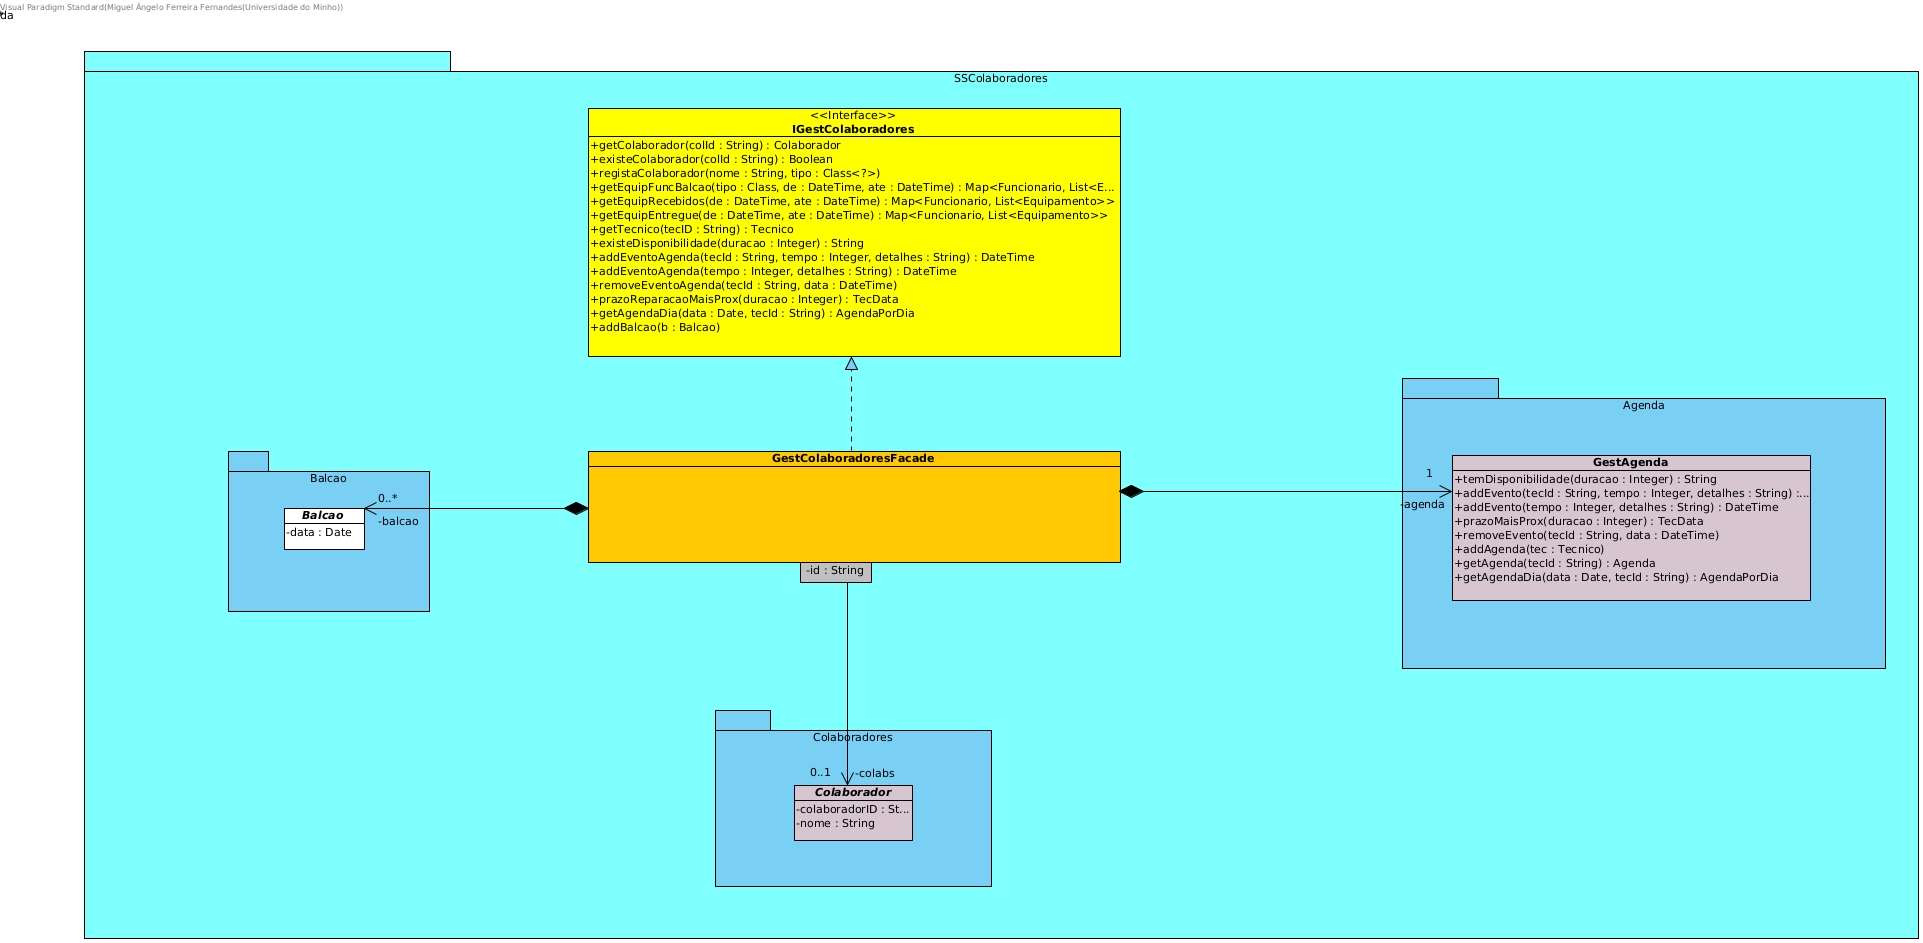
\includegraphics[scale=0.27]{SSColaboradores.jpg}
    \caption{SubSistema SSReparacoes \ref{sec:ss_colaboradores}}
\end{figure}

\end{document}